
\providecommand{\Fun}{\operatorname{Fun}}
\providecommand{\QCat}{\mathcal{Q}\mathcal{C}at}
\providecommand{\qcor}[1]{\ulcorner#1\urcorner}   %
\providecommand{\qcInt}{\mathbb{I}}   %
\providecommand{\PUpair}[5]{\tikz[baseline=-0.6ex,x=1.15em,y=0.95em]{%
  \node (PUa) at (0,0) {$#1$};%
  \node (PUb) at (3.6,0) {$#2$};%
  \draw[->] (0.65,0.38) to[bend left=12] node[above]{$\scriptstyle#3$} (2.95,0.38);%
  \node at (1.8,0) {$\scriptstyle\Downarrow#4$};%
  \draw[->] (0.65,-0.38) to[bend right=12] node[below]{$\scriptstyle#5$} (2.95,-0.38);}}

\section{逐点泛性质}\label{sec:pointwise-universal-properties}

在一个 $(\infty,1)$-\trCategory{}的\trInfinityCosmos{}中，\trTerminal{}%
∞-\trCategory{} $1$ 扮演着一个特殊角色，这一角色可以概括为如下口号：%
「诸\trUniversalProperty{}是逐点检测的」。在本节中，我们汇集起若干例示这一
口号的结果，它们的证明综合运用了综合技巧与解析技巧。

例如，第 1 章中的\cref{cor:exponential-ideal}陈述而附录 D 的推论 D.4.19 证明：%
诸\trQuasiCategory{}之间的诸\trFunctor{}之间的一个\trNaturalTransformation{}
\PUpair{X}{A}{f}{\alpha}{g}是一个自然同构，当且仅当它是一个\textbf{逐点同构}
（pointwise isomorphism），意即它的每一个分量
\tikz[baseline=-0.6ex,x=1.15em,y=0.95em]{%
  \node (PUa) at (0,0) {$1$};%
  \node (PUb) at (3.6,0) {$X$};%
  \node (PUc) at (7.2,0) {$A$};%
  \draw[->] (PUa) -- node[above]{$\scriptstyle x$} (PUb);%
  \draw[->] (4.25,0.38) to[bend left=12] node[above]{$\scriptstyle f$} (6.55,0.38);%
  \node at (5.4,0) {$\scriptstyle\Downarrow\alpha$};%
  \draw[->] (4.25,-0.38) to[bend right=12] node[below]{$\scriptstyle g$} (6.55,-0.38);}
是可逆的。从而：

\begin{lemma}\label{lem:pointwise-natural-isomorphism}
在一个 $(\infty,1)$-\trCategory{}的\trInfinityCosmos{}中，一个%
\trNaturalTransformation{}是一个自然同构，当且仅当它是一个逐点同构。
\end{lemma}

\begin{proof}
任何自然同构显然都是逐点同构。为证其逆，我们动用命题 10.2.1 与命题 10.3.1 的
2-范畴双等价 $(-)_{0}\colon\mathfrak{h}\mathcal{K}\Rightarrow\mathfrak{h}\QCat$。
设 \PUpair{X}{A}{f}{\alpha}{g} 是 $\mathfrak{h}\mathcal{K}$ 中的一个逐点自然
同构，并考虑诸底拟范畴之间的底\trNaturalTransformation{}
\PUpair{X_{0}}{A_{0}}{f_{0}}{\alpha_{0}}{g_{0}}。由构造，$X_{0}\cong\Fun(1,X)$
的顶点 $x$ 与 $X$ 的诸\trElement{}双射地对应，而这些分量
\begin{center}
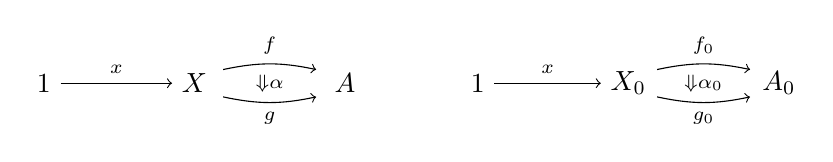
\begin{tikzpicture}[x=1.6em,y=1.3em]
  \node (a1) at (0,0) {$1$};
  \node (b1) at (3.4,0) {$X$};
  \node (c1) at (6.8,0) {$A$};
  \draw[->] (a1) -- node[above]{$\scriptstyle x$} (b1);
  \draw[->] (4.05,0.38) to[bend left=12] node[above]{$\scriptstyle f$} (6.15,0.38);
  \node at (5.1,0) {$\scriptstyle\Downarrow\alpha$};
  \draw[->] (4.05,-0.38) to[bend right=12] node[below]{$\scriptstyle g$} (6.15,-0.38);
  \node at (8.3,0) {$\leftrightsquigarrow$};
  \begin{scope}[shift={(9.8,0)}]
    \node (a2) at (0,0) {$1$};
    \node (b2) at (3.4,0) {$X_{0}$};
    \node (c2) at (6.8,0) {$A_{0}$};
    \draw[->] (a2) -- node[above]{$\scriptstyle x$} (b2);
    \draw[->] (4.05,0.38) to[bend left=12] node[above]{$\scriptstyle f_{0}$} (6.15,0.38);
    \node at (5.1,0) {$\scriptstyle\Downarrow\alpha_{0}$};
    \draw[->] (4.05,-0.38) to[bend right=12] node[below]{$\scriptstyle g_{0}$} (6.15,-0.38);
  \end{scope}
\end{tikzpicture}
\end{center}
在 $\mathrm{h}A\cong\mathrm{h}(A_{0})$ 中定义相应的箭头。于是，底%
\trNaturalTransformation{} $\alpha_{0}$ 在 $\mathfrak{h}\QCat$ 中也是一个逐点
自然同构，而推论 D.4.19 适用于证明 $\alpha_{0}$ 容有一个逆
\PUpair{X_{0}}{A_{0}}{g_{0}}{\alpha_{0}^{-1}}{f_{0}}。由命题 10.3.1 所建立的
局部等价 $\mathrm{h}\Fun(X,A)\Rightarrow\mathrm{h}\Fun(X_{0},A_{0})$ 的
全忠实性，这个 2-胞腔提升而定义一个逆\trNaturalTransformation{}
\PUpair{X}{A}{g}{\alpha^{-1}}{f}，见证 $\alpha$ 的可逆性。
\end{proof}

值得提请注意：\cref{lem:pointwise-natural-isomorphism}之证明中所用的宇宙论%
\trBiequivalence{} $(-)_{0}\colon\mathcal{K}\Rightarrow\QCat$ 的一个特殊性质。

\begin{observation}[论底拟范畴的\trElement]\label{obs:elements-of-underlying-qcat}
由推论 10.3.2(ii)，一个宇宙论\trBiequivalence{}
$F\colon\mathcal{K}\Rightarrow\mathcal{L}$ 在 $\mathcal{K}$ 中一个%
∞-\trCategory{} $A\in\mathcal{K}$ 的诸\trElement{}的同构类与 $\mathcal{L}$ 中
$FA\in\mathcal{L}$ 的诸\trElement{}的同构类之间诱导一个双射，而且事实上诱导%
诸\trHomotopyCategory{}的一个\trEquivalence{} $\mathrm{h}A\Rightarrow\mathrm{h}FA$
——后者的对象恰是这些元素（见练习 10.3.i）。特别地，任何\trElement{}
$x\colon 1\to FA$ 都自然同构于一个\trElement{} $Fa\colon 1\to FA$，后者是某个%
\trElement{} $a\colon 1\to A$ 的像。由于「逐点的」∞-范畴性概念——一个自然
同构诸分量的可逆性、一个\trCocartesianFibration{}诸纤维中\trTerminal{}元素
之拥有——在\trIsomorphism{}之下不变，故若 $A$ 在 $\mathcal{K}$ 中满足某个逐点
判据，则 $FA$ 在 $\mathcal{L}$ 中满足相应的逐点判据。
\end{observation}

但在 $(\infty,1)$-\trCategory{}的\trInfinityCosmos{}的情形中，命题 10.2.1 提供了一个宇宙论%
\trBiequivalence{} $(-)_{0}\colon\mathcal{K}\to\QCat$，它在∞-%
\trCategory{}的诸\trElement{}上双射地作用。由构造，$A_{0}\cong\Fun(1,A)$ 的
诸顶点与 $A$ 的诸\trElement{}双射地对应。从而，正如%
\cref{lem:pointwise-natural-isomorphism}之证明所例示的，「逐点的」性质甚至可
以更容易地转移。

借助\cref{lem:pointwise-natural-isomorphism}，我们可以证明：一个 $(\infty,1)$-%
\trCategory{}的\trInfinityCosmos{}中的一个\trIsofibration{}是\trSliceInfinityCosmos{}中的一个\trDiscrete{}对象，当且仅当它的诸纤维是\trDiscrete{}%
∞-\trCategory。由此可知：$(\infty,1)$-\trCategory{}的\trCocartesianFibration、%
\trCartesianFibration{}或\trTwoSidedFibration{}是\trDiscrete，当且仅当它们
拥有\trDiscrete{}纤维。

\begin{proposition}\label{prop:discrete-fibers-isofibration}
设 $p\colon E\twoheadrightarrow B$ 是一个 $(\infty,1)$-\trCategory{}的%
\trInfinityCosmos{} $\mathcal{K}$ 中的一个\trIsofibration。则 $p$ 作为
$\mathcal{K}_{/B}$ 的对象是\trDiscrete，当且仅当 $p$ 的诸纤维是 $\mathcal{K}$
中的\trDiscrete{}∞-\trCategory。
\end{proposition}

\begin{proof}
任何\trElement{} $b\colon 1\to B$ 诱导一个宇宙论\trFunctor{}
$b^{*}\colon\mathcal{K}_{/B}\to\mathcal{K}$，由第 1 章中的%
\cref{rem:cosmological-discrete-categories}它保持\trDiscrete{}∞-\trCategory。
于是，对任何\trInfinityCosmos{} $\mathcal{K}$，若
$p\colon E\twoheadrightarrow B$ 是 $\mathcal{K}_{/B}$ 中一个\trDiscrete{}%
对象，则它的诸纤维是\trDiscrete{}∞-\trCategory。

为证其逆，我们假设 $\mathcal{K}$ 是一个 $(\infty,1)$-\trCategory{}的%
\trInfinityCosmos{}并诉诸\cref{lem:pointwise-natural-isomorphism}。为证
$p\colon E\twoheadrightarrow B$ 在 $\mathcal{K}_{/B}$ 中是\trDiscrete，
我们必须论证：由如下\trPullback{}所定义的\trQuasiCategory
\begin{center}
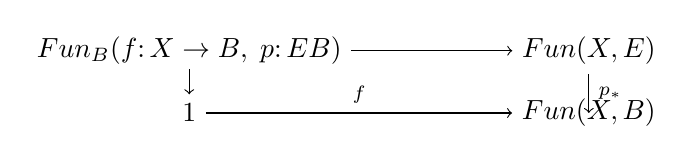
\begin{tikzpicture}[x=1.9em,y=1.5em]
  \node (tl) at (0,1.5) {$\Fun_{B}(f\colon X\to B,\; p\colon E\twoheadrightarrow B)$};
  \node (tr) at (7.6,1.5) {$\Fun(X,E)$};
  \node (bl) at (0,0) {$1$};
  \node (br) at (7.6,0) {$\Fun(X,B)$};
  \draw[->] (tl) -- (tr);
  \draw[->] (0,1.05) -- (0,0.45);
  \draw[->] (tr) -- node[right]{$\scriptstyle p_{*}$} (tr |- br);
  \draw[->] (bl) -- node[above]{$\scriptstyle f$} (br);
  \node at (1.15,0.95) {$\scriptstyle\lrcorner$};
\end{tikzpicture}
\end{center}
是一个\trKanComplex。由第 1 章中的\cref{cor:kan-groupoid}，只需证明其%
\trHomotopyCategory{}是一个\trGroupoid；为此我们动用第 3 章中的%
\cref{lem:smothering-pullback}的\trSmotheringFunctor
\[
\mathrm{h}\bigl(\Fun_{B}(f\colon X\to B,\; p\colon E\twoheadrightarrow B)\bigr)
  \longrightarrow 1\times_{\mathrm{h}\Fun(X,B)}\mathrm{h}\Fun(X,E)
\]
它特别地反射诸\trIsomorphism。$\mathrm{h}(\Fun_{B}(f,p))$ 的诸箭头由那些具有
如下性质的 1-\trSimplex{} $\alpha\colon e\to e'\in\Fun(X,E)$ 所表示：须化复合
$p\alpha\in\Fun(X,B)$ 是 $f$ 处的退化 1-\trSimplex。\footnote{这蕴含、但强于
如下性质：\trHomotopyTwoCategory{}中的须化复合等于 2-\trCell{} $\mathrm{id}_{f}$
（讨论见 3.6 节）。}由\cref{lem:pointwise-natural-isomorphism}，%
\trNaturalTransformation{} $\alpha\colon e\Rightarrow e'\in\mathrm{h}\Fun(X,E)$
是可逆的，当且仅当其对每个 $x\colon 1\to X$ 的分量 $\alpha_{x}$ 都是可逆的。
由于 1-\trSimplex{} $p\alpha$ 在 $\Fun(X,B)$ 中退化，1-\trSimplex{} $p\alpha_{x}$
在顶点 $fx\in\Fun(1,B)$ 处退化，这表明 $\alpha_{x}$ 落于 $fx\colon 1\to B$
之上的纤维中。由于 $p\colon E\twoheadrightarrow B$ 的诸纤维是\trDiscrete，
这就告诉我们 $\alpha_{x}$ 是可逆的，于是由%
\cref{lem:pointwise-natural-isomorphism}我们断定 $\alpha$ 可逆，如所宣称。
\end{proof}

我们接下来的这一系列结果表明：诸\trUniversalProperty{}可以在 $(\infty,1)$-%
\trCategory{}的诸\trInfinityCosmos{}中被逐点检测。关键技术配料是一个关于诸%
\trQuasiCategory{}的解析结果，风格承 Joyal 与 Lurie。

\begin{proposition}\label{prop:cocartesian-rari-terminal-elements}
诸\trQuasiCategory{}的一个\trCocartesianFibration{}
$q\colon E\twoheadrightarrow A$ 容有一个\trRightAdjoint\trRightInverse{}
$t\colon A\to E$，当且仅当对每个\trElement{} $a\colon 1\to A$，纤维 $E_{a}$
拥有一个\trTerminal{}元素。
\end{proposition}

\begin{proof}
由第 3 章中的\cref{lem:rajri-fibered-adjunction}，$q$ 的一个%
\trRightAdjoint\trRightInverse{}可以解读为在 $q\colon E\twoheadrightarrow A$
——视之为切片\trInfinityCosmos{} $\QCat_{/A}$ 中的一个对象——中定义一个%
\trTerminal{}元素。由第 3 章中的\cref{lem:fibered-adjunction-pullback-projection}(i)，
这个纤维化的\trAdjunction{}可以沿任何\trElement{} $a\colon 1\to A$ 拉回，
以在纤维 $E_{a}$ 中定义一个\trTerminal{}元素。

为证其逆，设 $ta\colon 1\to E_{a}$ 表示在\trElement{} $a\colon 1\to A$ 之上
的纤维 $E_{a}$ 中所选定的一个\trTerminal{}元素。引理 F.3.1 以一个\trLifting{}%
性质刻画诸\trQuasiCategory{}之间那些容有\trRightAdjoint\trRightInverse{}的%
\trIsofibration。在此情形中，只需证明：任何\trLifting{}问题
\begin{center}
\begin{tikzpicture}[x=1.7em,y=1.4em]
  \node (one) at (0,1.4) {$1$};
  \node (bd)  at (3.4,1.4) {$\partial\Delta[n]$};
  \node (E)   at (8.0,1.4) {$E$};
  \draw[->] (one) -- node[below]{$\scriptstyle\{n\}$} (bd);
  \draw[->] (bd) -- node[above]{$\scriptstyle y$} (E);
  \draw[->] (0.6,1.9) to[bend left=20] node[above]{$\scriptstyle ta$} (7.4,1.9);
  \draw[right hook->] (3.4,0.95) -- (3.4,0.4);
  \draw[->] (8.0,0.95) -- node[right]{$\scriptstyle q$} (8.0,0.4);
  \node (dn) at (3.4,0) {$\Delta[n]$};
  \node (A)  at (8.0,0) {$A$};
  \draw[->] (dn) -- node[below]{$\scriptstyle x$} (A);
  \draw[->,dashed] (3.85,0.25) -- (7.55,1.15);
\end{tikzpicture}
\end{center}
对 $n\ge 1$ 都有解。为此，考虑单纯映射
$k\colon\Delta[n]\times\Delta[1]\to\Delta[n]$，其在顶点上由
$k(i,0)\coloneqq i$ 与 $k(i,1)\coloneqq n$ 定义。复合
$xk\colon\Delta[n]\times\Delta[1]\to A$ 限制而定义一个映射
$xk\colon\partial\Delta[n]\times\Delta[1]\to A$，它表示一个 2-\trCell{}：由在
$\Delta[1]$ 的顶点 $\{1\}$ 处求值所定义的余定义域于 $a$ 处取常值，而其定义域沿
$y$ 穿过 $q$ 作分解。这给出一个新的\trLifting{}问题
\begin{center}
\begin{tikzpicture}[x=1.8em,y=1.4em]
  \node (tl) at (0,1.4) {$\partial\Delta[n]$};
  \node (tr) at (5.6,1.4) {$E$};
  \node (bl) at (0,0) {$\partial\Delta[n]\times\Delta[1]$};
  \node (br) at (5.6,0) {$A$};
  \draw[->] (tl) -- node[above]{$\scriptstyle y$} (tr);
  \draw[right hook->] (0,0.95) -- (0,0.45);
  \node at (-0.75,0.7) {$\scriptstyle i_{0}$};
  \draw[->,dashed] (1.0,0.25) -- (4.9,1.15);
  \node at (2.6,0.95) {$\scriptstyle z$};
  \draw[->] (tr) -- node[right]{$\scriptstyle q$} (tr |- br);
  \draw[->] (bl) -- node[below]{$\scriptstyle xk$} (br);
\end{tikzpicture}
\end{center}
引理 F.4.8 使我们能够求解它。由引理 F.4.8，提升 $z$ 表示 2-\trCell{} $\varkappa$
的一个 $q$-余笛卡尔提升 $\zeta$，这里 $\varkappa$ 由 $xk$ 的限制所表示：
\begin{center}
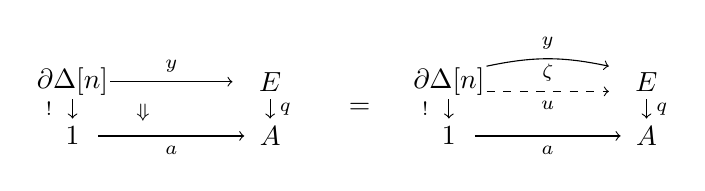
\begin{tikzpicture}[x=1.7em,y=1.4em]
  \node (a1) at (0,1.4) {$\partial\Delta[n]$};
  \node (b1) at (4.2,1.4) {$E$};
  \draw[->] (0.8,1.4) -- node[above]{$\scriptstyle y$} (3.4,1.4);
  \draw[->] (0,0.95) -- (0,0.45);
  \node at (-0.5,0.7) {$\scriptstyle !$};
  \node at (1.5,0.6) {$\scriptstyle\Downarrow\varkappa$};
  \draw[->] (4.2,0.95) -- node[right]{$\scriptstyle q$} (4.2,0.45);
  \node (c1) at (0,0) {$1$};
  \node (d1) at (4.2,0) {$A$};
  \draw[->] (0.55,0) -- node[below]{$\scriptstyle a$} (3.65,0);
  \node at (6.1,0.7) {$=$};
  \begin{scope}[shift={(8.0,0)}]
    \node (a2) at (0,1.4) {$\partial\Delta[n]$};
    \node (b2) at (4.2,1.4) {$E$};
    \draw[->] (0.8,1.8) to[bend left=12] node[above,pos=0.5]{$\scriptstyle y$} (3.4,1.8);
    \draw[->,dashed] (0.8,1.15) -- node[above,pos=0.5]{$\scriptstyle\zeta$}
      node[below,pos=0.5]{$\scriptstyle u$} (3.4,1.15);
    \draw[->] (0,0.95) -- (0,0.45);
    \node at (-0.5,0.7) {$\scriptstyle !$};
    \draw[->] (4.2,0.95) -- node[right]{$\scriptstyle q$} (4.2,0.45);
    \node (c2) at (0,0) {$1$};
    \node (d2) at (4.2,0) {$A$};
    \draw[->] (0.55,0) -- node[below]{$\scriptstyle a$} (3.65,0);
  \end{scope}
\end{tikzpicture}
\end{center}
由构造，右方所示 $q$-余笛卡尔提升的余定义域\trFunctor{}落入 $a$ 之上的纤维中。
现在，$\varkappa$ 在最终顶点 $\{n\}\colon 1\to\partial\Delta[n]$ 处的分量是
$\mathrm{id}_{a}$，故由第 5 章中的\cref{lem:isomorphism-stability}(ii)，表示
2-\trCell{} $\zeta\{n\}$ 的分量 $z\{n\}$ 是一个\trIsomorphism。特别地，
\trElement{} $u\{n\}\colon 1\to E$ \trIsomorphism{}于 $E_{a}$ 的\trTerminal{}%
元素 $y\{n\}=ta$，于是我们可以动用命题 F.1.1(vi) 的\trUniversalProperty{}把
$u$ 扩张成一个单纯形：
\begin{center}
\begin{tikzpicture}[x=1.8em,y=1.4em]
  \node (tl) at (0,1.4) {$\partial\Delta[n]$};
  \node (tr) at (4.8,1.4) {$E_{a}$};
  \draw[->] (tl) -- node[above]{$\scriptstyle u$} (tr);
  \draw[right hook->] (0,0.95) -- (0,0.45);
  \draw[->,dashed] (0.9,0.25) -- (4.0,1.15);
  \node at (2.7,0.95) {$\scriptstyle v$};
  \node (bl) at (0,0) {$\Delta[n]$};
\end{tikzpicture}
\end{center}
这份数据定义一个新的\trLifting{}问题
\begin{rveq}\label{eq:inductive-lifting-problem}
\begin{tikzpicture}[x=1.5em,y=1.5em]
  \node (tl) at (0,1.6) {$\partial\Delta[n]$};
  \node (tm) at (7.9,1.6) {$\partial\Delta[n]\times\Delta[1]\cup\Delta[n]\times\{1\}$};
  \node (tr) at (15.2,1.6) {$E$};
  \node (bl) at (0,0) {$\Delta[n]$};
  \node (bm) at (7.9,0) {$\Delta[n]\times\Delta[1]$};
  \node (br) at (15.2,0) {$A$};
  \draw[right hook->] (1.5,1.6) -- node[below]{$\scriptstyle i_{0}$} (4.3,1.6);
  \draw[->] (11.6,1.6) -- node[above]{$\scriptstyle z\cup v$} (14.0,1.6);
  \draw[right hook->] (1.2,0) -- node[below]{$\scriptstyle i_{0}$} (4.5,0);
  \draw[->] (11.4,0) -- node[above]{$\scriptstyle xk$} (14.0,0);
  \draw[right hook->] (0,1.1) -- (0,0.5);
  \draw[right hook->] (7.9,1.1) -- (7.9,0.5);
  \draw[->] (15.2,1.1) -- node[right]{$\scriptstyle q$} (15.2,0.5);
  \draw[->] (0.9,2.5) to[bend left=14] node[above]{$\scriptstyle y$} (14.3,2.5);
  \draw[->] (0.9,-0.9) to[bend right=14] node[below]{$\scriptstyle x$} (14.3,-0.9);
\end{tikzpicture}
\end{rveq}
我们按归纳法求解它：从含有 $\Delta[n]\times\{1\}$ 之面的那个
$(n+1)$-\trSimplex{}开始，为 $\Delta[n]\times\Delta[1]$ 中未出现于
$\partial\Delta[n]\times\Delta[1]\cup\Delta[n]\times\{1\}$ 的那 $n+1$ 个
$(n+1)$-\trSimplex{}逐一选取提升。除最后一个外，其余都可以借助对%
\trIsofibration{} $q$ 提升内\trHorn{}来实现。对于最后的

那个\trSimplex，我们必须求解一个外\trHorn{}\trLifting{}问题
\begin{center}
\begin{tikzpicture}[x=1.7em,y=1.4em]
  \node (d1) at (0,1.4) {$\Delta[1]$};
  \node (lh) at (5.0,1.4) {$\Lambda^{n+1}[n+1]$};
  \node (E)  at (9.8,1.4) {$E$};
  \draw[right hook->] (0.85,1.4) -- node[below]{$\scriptstyle\{n,n+1\}$} (3.3,1.4);
  \draw[->] (6.9,1.4) -- (8.5,1.4);
  \draw[->] (0.7,2.1) to[bend left=14] node[above,pos=0.5]{$\scriptstyle z\{n\}$} (9.1,2.1);
  \draw[right hook->] (5.0,0.95) -- (5.0,0.45);
  \draw[->] (9.8,0.95) -- node[right]{$\scriptstyle q$} (9.8,0.45);
  \node (dn) at (5.0,0) {$\Delta[n+1]$};
  \node (A)  at (9.8,0) {$A$};
  \draw[->] (dn) -- (A);
  \draw[->,dashed] (6.4,0.25) -- (9.2,1.15);
\end{tikzpicture}
\end{center}
但在此情形中，外\trHorn{}的最后一条边是\trIsomorphism{} $z\{n\}$，故第 1 章中的%
\cref{prop:special-outer-horn-lifting}也容许其求解。于是，提升
\eqref{eq:inductive-lifting-problem}限制而定义出原\trLifting{}问题所求的解，
这就证明了 $q\colon E\twoheadrightarrow A$ 容有一个\trRightAdjoint\trRightInverse。
\end{proof}

经由\cref{lem:opposite-qcat-biequivalence}的宇宙论\trBiequivalence{}
$(-)^{\mathrm{op}}\colon\QCat\simeq\QCat^{\mathrm{co}}$，
\cref{prop:cocartesian-rari-terminal-elements}之证明可以对偶化，以证明：诸%
\trQuasiCategory{}的一个\trCartesianFibration{}容有一个%
\trLeftAdjoint\trRightInverse，当且仅当每条纤维拥有一个\trInitial{}元素
（见\cref{ex:cartesian-lari-initial-elements}）。

\cref{prop:cocartesian-rari-terminal-elements}之证明颇倚重「解析的」技巧。
尽管如此，其结论可转移到任何\trBiequivalence{}于诸\trQuasiCategory{}的%
\trInfinityCosmos{}的\trInfinityCosmos。

\begin{proposition}\label{prop:pointwise-terminal-cocartesian-rari}
在一个 $(\infty,1)$-\trCategory{}的\trInfinityCosmos{}中，一个%
\trCocartesianFibration{} $q\colon E\twoheadrightarrow A$ 容有一个%
\trRightAdjoint\trRightInverse{} $t\colon A\to E$，当且仅当对每个\trElement{}
$a\colon 1\to A$，纤维 $E_{a}$ 拥有一个\trTerminal{}元素。
\end{proposition}

\begin{proof}
「带\trRightAdjoint\trRightInverse{}的\trIsofibration{}之诸纤维容有%
\trTerminal{}元素」这一方向的论证，与\cref{prop:cocartesian-rari-terminal-elements}
之证明中所给者相同。为证其逆，设 $q\colon E\twoheadrightarrow A$ 是一个
$(\infty,1)$-\trCategory{}的\trInfinityCosmos{} $\mathcal{K}$ 中的一个%
\trCocartesianFibration，带有如下性质：对底的每个\trElement{} $a\colon 1\to A$，
纤维 $E_{a}$ 拥有一个\trTerminal{}元素。由命题 10.2.1，我们可以动用底拟范畴%
\trBiequivalence{} $(-)_{0}\colon\mathcal{K}\Rightarrow\QCat$ 而断言：一旦证得
$q_{0}\colon E_{0}\to A_{0}$ 满足%
\cref{prop:cocartesian-rari-terminal-elements}的前提，$q$ 便容有一个%
\trRightAdjoint\trRightInverse。

宇宙论\trFunctor{}保持\trCocartesianFibration，故底映射
$q_{0}\colon E_{0}\to A_{0}$ 定义诸\trQuasiCategory{}的一个%
\trCocartesianFibration。由\cref{obs:elements-of-underlying-qcat}，底拟范畴
$A_{0}$ 的诸\trElement{}与∞-\trCategory{} $A$ 的诸\trElement{}双射地对应。由
假设，对每个\trElement{} $a\colon 1\to A$，∞-\trCategory{} $E_{a}$ 容有一个%
\trTerminal{}元素，故由命题 10.1.4，底拟范畴 $(E_{a})_{0}$ 亦然。如此我们看到：
诸\trQuasiCategory{}的\trCocartesianFibration{}
$q_{0}\colon E_{0}\to A_{0}$ 的每条纤维都容有一个\trTerminal{}%
元素。由\cref{prop:cocartesian-rari-terminal-elements}，$q_{0}$ 容有一个%
\trRightAdjoint\trRightInverse。如今由命题 10.3.6，我们可以断言
$q\colon E\twoheadrightarrow A$ 在 $\mathcal{K}$ 中容有一个%
\trRightAdjoint\trRightInverse，如所望。
\end{proof}

\cref{prop:pointwise-terminal-cocartesian-rari}的一个重要特例，证明了围绕
命题 4.1.6 的讨论中所许诺的一个结果：在一个 $(\infty,1)$-\trCategory{}的%
\trInfinityCosmos{}中，一个\trFunctor{} $f\colon B\to A$ 容有一个右伴随，恰当
对每个\trElement{} $a\colon 1\to A$，∞-\trCategory{}
$\mathrm{Hom}_{A}(f,a)$ 容有一个\trTerminal{}元素之时：即余单位分量
$\qcor{\varepsilon a}\colon 1\to\mathrm{Hom}_{A}(f,a)$。用 Mac Lane
[81, \S III.1] 的术语来说，这条\trUniversalProperty{}把 $\qcor{\varepsilon a}$
展示为从\trFunctor{} $f$ 到\trElement{} $a$ 的一支「泛箭头」。

\begin{corollary}\label{cor:right-adjoint-terminal-elements}
在一个 $(\infty,1)$-\trCategory{}的\trInfinityCosmos{}中，一个\trFunctor{}
$f\colon B\to A$ 容有一个右伴随，当且仅当对每个\trElement{} $a\colon 1\to A$，
\trCommaInfinityCategory{} $\mathrm{Hom}_{A}(f,a)$ 容有一个\trTerminal{}元素。
\end{corollary}

\begin{proof}
命题 4.1.6 表明：在任何\trInfinityCosmos{}中，$f\colon B\to A$ 容有一个右伴随，
当且仅当 $\mathrm{Hom}_{A}(f,A)$ 容有 $A$ 上的一个\trTerminal{}元素——意即
$p_{1}\colon\mathrm{Hom}_{A}(f,A)\twoheadrightarrow A$ 容有一个%
\trRightAdjoint\trRightInverse。由第 5 章中的\cref{cor:comma-domain-projections}，
这个\trFunctor{}是一个\trCocartesianFibration，故%
\cref{prop:pointwise-terminal-cocartesian-rari}告诉我们：$p_{1}$ 容有一个%
\trRightAdjoint\trRightInverse，当且仅当每条纤维 $\mathrm{Hom}_{A}(f,a)$
容有一个\trTerminal{}元素。
\end{proof}

\cref{prop:pointwise-terminal-cocartesian-rari}蕴含：$(\infty,1)$-%
\trCategory{}之间的诸\trModule{}容有一个类似的「逐点」可表示性条件，它刻画
那些在定义 7.4.7 的意义下被一个\trFunctor{}协变地或反变地表示的\trModule。

\begin{corollary}\label{cor:pointwise-covariant-representability}
在一个 $(\infty,1)$-\trCategory{}的\trInfinityCosmos{}中，一个\trModule{}
$A\xrightarrow{E}B$ 是协变表示的，当且仅当对每个\trElement{} $a\colon 1\to A$，
\trModule{} $1\xrightarrow{E(1,a)}B$ 是协变表示的；而后一情形成立，当且仅当每个
∞-\trCategory{} $E(1,a)$ 容有一个\trTerminal{}元素。
\end{corollary}

\begin{proof}
由第 8 章中的\cref{prop:detect-representable-modules}，由 $(q,p)\colon E\twoheadrightarrow A\times B$ 所编码的%
\trModule{} $A\xrightarrow{E}B$ 是协变表示的，当且仅当其左腿
$q\colon E\twoheadrightarrow A$ 容有一个\trRightAdjoint\trRightInverse{}
$r\colon A\to E$，此时 $E\cong\mathrm{Hom}_{B}(B,pr)$。由引理 7.4.3，左腿
$q\colon E\twoheadrightarrow A$ 定义一个\trCocartesianFibration，故由%
\cref{prop:pointwise-terminal-cocartesian-rari}，$q$ 容有一个%
\trRightAdjoint\trRightInverse，当且仅当在每个\trElement{} $a\colon 1\to A$
之上的纤维 $E_{a}$ 容有一个\trTerminal{}元素。对每个\trElement{}
$a\colon 1\to A$，\trModule{} $1\xrightarrow{E(1,a)}B$ 由沿
$a\times\mathrm{id}\colon 1\times B\to A\times B$ 取\trPullback{}而给出，从而%
\trIsomorphism{}于\trModule{} $1\xrightarrow{E_{a}}B$。再次应用第 8 章中的%
\cref{prop:detect-representable-modules}：
这个\trModule{}被某个\trElement{}协变表示，当且仅当 $!\colon E_{a}\to 1$
容有一个\trRightAdjoint\trRightInverse，而后一情形成立，当且仅当∞-%
\trCategory{} $E_{a}\cong E(1,a)$ 容有一个\trTerminal{}元素。
\end{proof}

我们的下一条结果关乎绝对提升图——定义 2.3.8 用它们来定义一个图表族的%
\trLimit{}或\trColimit。就陈述诸如命题 2.3.15 之类的结果而言，考虑诸图表的族
而非单个图表，自有其一番雅致；但逐一地确立\trLimit{}与\trColimit{}的存在性
——每次一个图表——同样有用。在 $(\infty,1)$-\trCategory{}的诸%
\trInfinityCosmos{}中，这类约化是可能的，其凭据如下：

\begin{proposition}\label{prop:absolute-right-lifting-pointwise}
在一个 $(\infty,1)$-\trCategory{}的\trInfinityCosmos{}中：
\begin{enumerate}[label=(\roman*)]
\item 一个\trFunctor{} $g\colon C\to A$ 穿过一个\trFunctor{} $f\colon B\to A$
  容有一个\trAbsoluteRightLifting，当且仅当对一切\trElement{} $c\colon 1\to C$，%
  \trCommaInfinityCategory{} $\mathrm{Hom}_{A}(f,gc)$ 容有一个\trTerminal{}元素。
\item 如左下方的三角形
\begin{center}
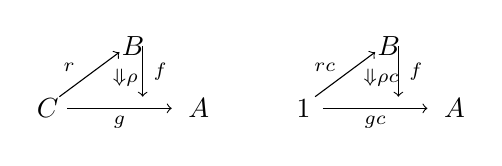
\begin{tikzpicture}[x=1.4em,y=1.4em]
  \node (b) at (2.2,1.6) {$B$};
  \node (c) at (0,0) {$C$};
  \node (a) at (3.9,0) {$A$};
  \draw[->] (0.3,0.3) -- (1.85,1.45);
  \node at (0.55,1.05) {$\scriptstyle r$};
  \node at (2.0,0.78) {$\scriptstyle\Downarrow\rho$};
  \draw[->] (2.45,1.6) -- (2.45,0.3);
  \node at (2.9,0.95) {$\scriptstyle f$};
  \draw[->] (0.5,0) -- (3.2,0);
  \node at (1.85,-0.36) {$\scriptstyle g$};
  \begin{scope}[shift={(6.6,0)}]
    \node (b2) at (2.2,1.6) {$B$};
    \node (c2) at (0,0) {$1$};
    \node (a2) at (3.9,0) {$A$};
    \draw[->] (0.3,0.3) -- (1.85,1.45);
    \node at (0.55,1.05) {$\scriptstyle rc$};
    \node at (2.0,0.78) {$\scriptstyle\Downarrow\rho c$};
    \draw[->] (2.45,1.6) -- (2.45,0.3);
    \node at (2.9,0.95) {$\scriptstyle f$};
    \draw[->] (0.5,0) -- (3.2,0);
    \node at (1.85,-0.36) {$\scriptstyle gc$};
  \end{scope}
\end{tikzpicture}
\end{center}
  显示 $r$ 为 $g$ 穿过 $f$ 的一个\trAbsoluteRightLifting，当且仅当对一切\trElement{}
  $c\colon 1\to C$，如右上方的受限三角形显示 $rc$ 为 $gc$ 穿过 $f$ 的一个%
  \trAbsoluteRightLifting。
\item 一个\trFunctor{} $g\colon C\to A$ 穿过一个\trFunctor{} $f\colon B\to A$
  容有一个\trAbsoluteRightLifting，当且仅当对一切\trElement{} $c\colon 1\to C$，$gc$ 穿过
  $f$ 都存在一个如下左方所示的\trAbsoluteRightLifting
\begin{center}
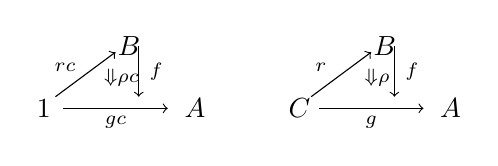
\begin{tikzpicture}[x=1.4em,y=1.4em]
  \node (b) at (2.2,1.6) {$B$};
  \node (c) at (0,0) {$1$};
  \node (a) at (3.9,0) {$A$};
  \draw[->] (0.3,0.3) -- (1.85,1.45);
  \node at (0.55,1.05) {$\scriptstyle rc$};
  \node at (2.0,0.78) {$\scriptstyle\Downarrow\rho c$};
  \draw[->] (2.45,1.6) -- (2.45,0.3);
  \node at (2.9,0.95) {$\scriptstyle f$};
  \draw[->] (0.5,0) -- (3.2,0);
  \node at (1.85,-0.36) {$\scriptstyle gc$};
  \begin{scope}[shift={(6.6,0)}]
    \node (b2) at (2.2,1.6) {$B$};
    \node (c2) at (0,0) {$C$};
    \node (a2) at (3.9,0) {$A$};
    \draw[->] (0.3,0.3) -- (1.85,1.45);
    \node at (0.55,1.05) {$\scriptstyle r$};
    \node at (2.0,0.78) {$\scriptstyle\Downarrow\rho$};
    \draw[->] (2.45,1.6) -- (2.45,0.3);
    \node at (2.9,0.95) {$\scriptstyle f$};
    \draw[->] (0.5,0) -- (3.2,0);
    \node at (1.85,-0.36) {$\scriptstyle g$};
  \end{scope}
\end{tikzpicture}
\end{center}
  在此情形，如右上方 $g$ 穿过 $f$ 的\trAbsoluteRightLifting{}的诸分量\trIsomorphism{}于相应的
  逐点绝对提升：$r_{c}\cong rc$ 且 $\rho_{c}\cong\rho c$。
\end{enumerate}
\end{proposition}

\begin{proof}
第 3 章中的\cref{thm:trio-bijection}与\cref{thm:right-representability}表明：在任何\trInfinityCosmos{}中，一个\trFunctor{}
$g\colon C\to A$ 穿过 $f\colon B\to A$ 容有一个右提升，当且仅当余定义域投影%
\trFunctor{} $p_{1}\colon\mathrm{Hom}_{A}(f,g)\twoheadrightarrow C$ 容有一个%
\trRightAdjoint\trRightInverse。由第 5 章中的\cref{cor:comma-domain-projections}，
这个\trFunctor{}是一个\trCocartesianFibration。%
\cref{prop:pointwise-terminal-cocartesian-rari}证明：
在一个 $(\infty,1)$-\trCategory{}的\trInfinityCosmos{}中，
$p_{1}\colon\mathrm{Hom}_{A}(f,g)\twoheadrightarrow C$ 容有一个%
\trRightAdjoint\trRightInverse，当且仅当在\trElement{} $c\colon 1\to C$ 之上
的每条纤维 $\mathrm{Hom}_{A}(f,gc)$ 容有一个\trTerminal{}元素。这就证明了
第一款。

由于绝对提升图在限制下稳定，任何如左上方所示的\trAbsoluteRightLifting{}图表都限制而定义一个
逐点的\trAbsoluteRightLifting{}图表，如右上方所示。为证其逆，设 $(rc,\rho c)$ 对任意%
\trElement{} $c\colon 1\to C$ 都定义 $gc$ 穿过 $f$ 的一个\trAbsoluteRightLifting。由第 3 章中的%
\cref{thm:right-representability}，由此可知每个\trCommaInfinityCategory{} $\mathrm{Hom}_{A}(f,gc)$ 都
拥有一个\trTerminal{}元素，于是由 (i)，$g\colon C\to A$ 必定容有穿过
$f\colon B\to A$ 的一个\trAbsoluteRightLifting{} $(s,\sigma)$。据其\trUniversalProperty，对
$(r,\rho)$ 经由一支 2-\trCell{} $\tau\colon r\Rightarrow s$ 穿过 $(s,\sigma)$
作分解，使得 $\rho=\sigma\cdot f\tau$。由于 $(rc,\rho c)$ 与 $(sc,\sigma c)$
都是\trAbsoluteRightLifting{}图表，我们知道每个分量 $\tau c$ 都是\trIsomorphism。从而，由%
\cref{lem:pointwise-natural-isomorphism}，$\tau$ 是一个\trIsomorphism，于是
$(r,\rho)$ 也是一个\trAbsoluteRightLifting{}图表，如所望。

第三款是对前两款的一个便利总结。若 $gc$ 穿过 $f$ 容有一个\trAbsoluteRightLifting，则
$\mathrm{Hom}_{A}(f,gc)$ 拥有一个\trTerminal{}元素，而 (i) 保证 $g$ 穿过 $f$
的某个\trAbsoluteRightLifting{}存在。$(r,\rho)$ 在 $c$ 处的分量定义 $gc$ 穿过 $f$ 的第二个%
\trAbsoluteRightLifting，从而诱导出所宣称的那些\trIsomorphism。
\end{proof}

作为一条推论，我们可以证成注 2.3.9 中所作的断言。

\begin{corollary}\label{cor:pointwise-limits-adjoint}
在一个 $(\infty,1)$-\trCategory{}的\trInfinityCosmos{}中，若 $A$ 是一个对形状
$J$ 的每个图表 $d\colon 1\to A^{J}$ 都容有\trLimit{}的∞-\trCategory，则 $A$
容有形状 $J$ 的一切\trLimit：也就是说，常值图表\trFunctor{}容有一个右伴随
\begin{center}
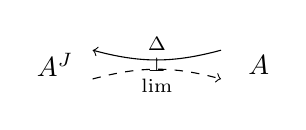
\begin{tikzpicture}[x=1.6em,y=1.3em]
  \node (AJ) at (0,0) {$A^{J}$};
  \node (A)  at (4.6,0) {$A$};
  \draw[->] (3.75,0.4) to[bend left=15] node[above]{$\scriptstyle\Delta$} (0.85,0.4);
  \node at (2.3,0) {$\scriptstyle\perp$};
  \draw[->,dashed] (0.85,-0.4) to[bend left=15] node[below]{$\scriptstyle\lim$} (3.75,-0.4);
\end{tikzpicture}
\end{center}
\end{corollary}

\begin{proof}
由\cref{prop:absolute-right-lifting-pointwise}(iii)，\trFunctor{}
$\mathrm{id}\colon A^{J}\to A^{J}$ 穿过 $\Delta\colon A\to A^{J}$ 容有一个%
\trAbsoluteRightLifting，当且仅当每个图表 $d\colon 1\to A^{J}$ 穿过 $\Delta\colon A\to A^{J}$
都容有一个\trAbsoluteRightLifting。由定义 2.3.8，后一条件编码了「$A$ 容有图表 $d$ 的一个%
\trLimit」之所指；而由引理 2.3.7，前一条件编码了「$\Delta\colon A\to A^{J}$
容有一个右伴随」之所指。
\end{proof}

\cref{prop:absolute-right-lifting-pointwise}(ii) 的另一个证明是可能的。由第 3 章中的%
\cref{thm:trio-bijection}，一支 2-\trCell{} $\rho\colon fr\Rightarrow g$ 定义一个\trAbsoluteRightLifting，当且
仅当诱导\trFunctor{}
$\qcor{\rho}\colon\mathrm{Hom}_{B}(B,r)\to\mathrm{Hom}_{A}(f,g)$ 是居于
$C\times B$ 之上的一个\trFiberedEquivalence。正如我们现在将要发现的，在
$(\infty,1)$-\trCategory{}的诸\trInfinityCosmos{}中，诸余/笛卡尔纤维化之间或
诸\trModule{}之间的\trEquivalence{}可以逐纤维地检测。正如构造余笛卡尔纤维化的%
\trRightAdjoint\trRightInverse{}时的策略一样，我们首先借助解析技巧对诸%
\trQuasiCategory{}证明这一结果。另类的解析证明可见于文献 [78, 3.3.1.5] 与
[5, 2.9]。随后我们动用\trModelIndependence{}断言：同样的结果在任意的
$(\infty,1)$-\trCategory{}的诸\trInfinityCosmos{}中成立。

\begin{proposition}\label{prop:fiberwise-equivalence-cartesian-functor}
诸\trQuasiCategory{}的\trCocartesianFibration{}之间的一个\trCartesianFunctor
\begin{center}
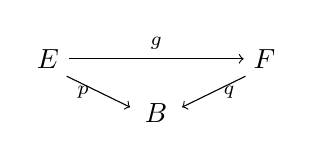
\begin{tikzpicture}[x=1.7em,y=1.4em]
  \node (E) at (0,1.4) {$E$};
  \node (F) at (4.6,1.4) {$F$};
  \node (B) at (2.3,0) {$B$};
  \draw[->] (E) -- node[above]{$\scriptstyle g$} (F);
  \draw[->] (0.4,0.95) -- node[left,pos=0.5]{$\scriptstyle p$} (1.75,0.15);
  \draw[->] (4.2,0.95) -- node[right,pos=0.5]{$\scriptstyle q$} (2.85,0.15);
\end{tikzpicture}
\end{center}
是一个\trFiberedEquivalence，当且仅当它是一个逐纤维等价，意即对每个\trElement{}
$b\colon 1\to B$，诱导的纤维间\trFunctor{} $g_{b}\colon E_{b}\to F_{b}$ 是一个%
\trEquivalence。
\end{proposition}

注意「纤维化等价」——$B$ 之上的\trEquivalence——与「逐纤维等价」——在 $B$
的诸\trElement{}之上的诸纤维上诱导\trEquivalence{}的映射——这两个术语之间的
微妙差别。本结果与紧随其后的\cref{prop:fiberwise-equivalence-cosmos}一道
表明：事实上，在
$(\infty,1)$-\trCategory{}的诸\trInfinityCosmos{}中，这两个概念对%
\trCartesianFunctor{}而言重合。

\begin{proof}
\trFiberedEquivalence{}在到纤维的拉回下稳定，故实质内容在于逆蕴含：任何在%
\trCocartesianFibration{}之间诱导逐纤维等价的\trCartesianFunctor{}都必然是一
个\trEquivalence。

这个\trCartesianFunctor{} $g$ 可以在切片 $\QCat_{/B}$ 中分解为一个%
\trEquivalence{}后接一个\trIsofibration。由第 5 章中的%
\cref{cor:equivalence-invariance}，该分解的中间对象仍是一个%
\trCocartesianFibration，而从这个中间对象出发、指向 $q\colon F\twoheadrightarrow B$
的\trIsofibration{}仍是一个\trCartesianFunctor。用与之\trEquivalence{}的%
\trCocartesianFibration{}替换 $p\colon E\twoheadrightarrow B$ 之后，因此只需
假设 $g\colon E\twoheadrightarrow F$ 既是一个\trIsofibration{}又是一个%
\trCartesianFunctor，\footnote{原书此处印作「$g\colon E\twoheadrightarrow B$」；
按上下文 $g$ 之余定义域为 $F$（见本条首图），疑为「$E\twoheadrightarrow F$」
之误，此处径改。——译者注}并设定每个诱导映射
$g_{b}\colon E_{b}\twoheadrightarrow F_{b}$ 都是一个\trTrivialFibration。在
这些假设下，我们必须证明 $g$ 自身是一个\trTrivialFibration。

为此，设给定一个\trLifting{}问题
\begin{center}
\begin{tikzpicture}[x=1.8em,y=1.4em]
  \node (tl) at (0,1.4) {$\partial\Delta[n]$};
  \node (tr) at (4.6,1.4) {$E$};
  \node (bl) at (0,0) {$\Delta[n]$};
  \node (br) at (4.6,0) {$F$};
  \draw[->] (tl) -- node[above]{$\scriptstyle e$} (tr);
  \draw[right hook->] (0,0.95) -- (0,0.45);
  \draw[->] (tr) -- node[right]{$\scriptstyle g$} (br);
  \draw[->] (bl) -- node[below]{$\scriptstyle f$} (br);
\end{tikzpicture}
\end{center}
于 $b\colon\Delta[n]\to B$ 之上。考虑收缩图表
\begin{center}
\begin{tikzpicture}[x=1.6em,y=1.3em]
  \node (a) at (0,1.6) {$\Delta[n]$};
  \node (b) at (6.2,1.6) {$\Delta[n]\times\Delta[1]$};
  \node (c) at (13.0,1.6) {$\Delta[n]$};
  \draw[->] (1.1,1.6) -- node[above]{$\scriptstyle\mathrm{id}\times\{0\}$} (3.4,1.6);
  \draw[->] (9.0,1.6) -- node[above]{$\scriptstyle r$} (11.3,1.6);
  \node at (1.0,0.55) {$\scriptstyle i\longmapsto(i,0)$};
  \node at (7.6,0.35) {$\scriptstyle(i,j)\longmapsto$};
  \node at (10.6,0.6) {$\scriptstyle\left\{\begin{array}{ll}i & \text{若 } j=0\\ n & \text{若 } j=1\end{array}\right.$};
\end{tikzpicture}
\end{center}

并选取一个逐点的 $p$-余笛卡尔提升
\begin{center}
\begin{tikzpicture}[x=1.9em,y=1.4em]
  \node (tl) at (0,1.4) {$\partial\Delta[n]\times\{0\}$};
  \node (tr) at (6.6,1.4) {$E$};
  \node (bl) at (0,0) {$\partial\Delta[n]\times\Delta[1]$};
  \node (br) at (6.6,0) {$B$};
  \draw[->] (tl) -- node[above]{$\scriptstyle e$} (tr);
  \draw[right hook->] (0,0.95) -- (0,0.45);
  \draw[->,dashed] (2.1,0.25) -- (5.8,1.15);
  \node at (3.5,0.95) {$\scriptstyle\chi$};
  \draw[->] (tr) -- node[right]{$\scriptstyle p$} (br);
  \draw[->] (bl) -- node[below]{$\scriptstyle br$} (br);
\end{tikzpicture}
\end{center}
如引理 F.4.8 所容许者。施加 $g$，我们得到一个空心柱面
\[
\partial\Delta[n]\times\Delta[1]\xrightarrow{\;\chi\;}E\xrightarrow{\;g\;}F
\]
由于 $g$ 是一个\trCartesianFunctor{}而 $\chi$ 是逐点 $p$-余笛卡尔的，故 $g\chi$
是逐点 $q$-余笛卡尔的。现在，由构造，单纯形
$f\colon\Delta[n]\times\{0\}\to F$ 在二者均有定义的子集
$\partial\Delta[n]\times\{0\}$ 上与 $g\chi\colon\Delta[n]\times\Delta[1]\to F$
相合。从而二者在其定义域之并上拼合成一个良定的单纯映射，于是为我们提供了第二
个\trLifting{}问题：
\begin{center}
\begin{tikzpicture}[x=1.9em,y=1.4em]
  \node (tl) at (0,1.4) {$\Delta[n]\times\{0\}\cup\Delta[n]\times\Delta[1]$};
  \node (tr) at (8.6,1.4) {$F$};
  \node (bl) at (0,0) {$\Delta[n]\times\Delta[1]$};
  \node (br) at (8.6,0) {$B$};
  \draw[->] (tl) -- node[above]{$\scriptstyle f\cup g\chi$} (tr);
  \draw[right hook->] (0,0.95) -- (0,0.45);
  \draw[->,dashed] (2.6,0.25) -- (7.8,1.15);
  \node at (4.4,0.95) {$\scriptstyle\rho$};
  \draw[->] (tr) -- node[right]{$\scriptstyle q$} (br);
  \draw[->] (bl) -- node[below]{$\scriptstyle br$} (br);
\end{tikzpicture}
\end{center}
它可以再度求解——由引理 F.4.8——给出一个逐点的 $q$-余笛卡尔提升 $\rho$。现在
注意：收缩 $r\colon\Delta[n]\times\Delta[1]\to\Delta[n]$ 被构造成把子集
$\Delta[n]\times\{1\}$ 映到顶点 $\{n\}$ 上，由此可知，$n$-\trSimplex
\[
\Delta[n]\times\{1\}\hookrightarrow\Delta[n]\times\Delta[1]\xrightarrow{\;br\;}B
\]
是最终顶点 $b_{n}\coloneqq b\cdot\{n\}$ 的一个退化像。现在观察到：柱面 $\chi$
与 $\rho$ 被定义为居于 $br\colon\Delta[n]\times\Delta[1]\to B$ 之上，故受限
映射
\[
\begin{gathered}
\partial\Delta[n]\times\{1\}\hookrightarrow\Delta[n]\times\Delta[1]
  \xrightarrow{\;\chi\;}E\\
\Delta[n]\times\{1\}\hookrightarrow\Delta[n]\times\Delta[1]
  \xrightarrow{\;\rho\;}F
\end{gathered}
\]
分别落入 $p$ 与 $q$ 的纤维 $E_{b_{n}}$ 与 $F_{b_{n}}$ 之中。于是，$\chi$ 与
$\rho$ 定义一个\trLifting{}问题
\begin{center}
\begin{tikzpicture}[x=1.8em,y=1.4em]
  \node (tl) at (0,1.4) {$\partial\Delta[n]$};
  \node (tr) at (5.0,1.4) {$E_{b_{n}}$};
  \node (bl) at (0,0) {$\Delta[n]$};
  \node (br) at (5.0,0) {$F_{b_{n}}$};
  \draw[->] (tl) -- node[above]{$\scriptstyle\chi\vert_{\{1\}}$} (tr);
  \draw[right hook->] (0,0.95) -- (0,0.45);
  \draw[->,dashed] (0.9,0.25) -- (4.2,1.15);
  \node at (2.3,0.95) {$\scriptstyle\gamma$};
  \draw[double,->] (tr) -- node[right]{$\scriptstyle g_{b_{n}}$} (br);
  \draw[->] (bl) -- node[below]{$\scriptstyle\rho\vert_{\{1\}}$} (br);
\end{tikzpicture}
\end{center}

它可以求解，因为右侧的纤维间映射按假设是一个\trTrivialFibration。现在，左上
三角形告诉我们：$\chi$ 与 $\gamma$ 在二者均有定义的子集
$\partial\Delta[n]\times\{1\}$ 上相合。于是，这些映射拼合而给出定义域之并上
的一个良定的单纯映射——即下方图表右侧那个\trLifting{}问题中画为上横边的
那个映射：
\begin{center}
\begin{tikzpicture}[x=1.8em,y=1.5em]
  \node (a) at (0,1.6) {$\partial\Delta[n]\times\{0\}$};
  \node (b) at (7.4,1.6) {$\Delta[n]\times\{1\}\cup\partial\Delta[n]\times\Delta[1]$};
  \node (c) at (15.0,1.6) {$E$};
  \node (d) at (0,0) {$\Delta[n]\times\{0\}$};
  \node (e) at (7.4,0) {$\Delta[n]\times\Delta[1]$};
  \node (f) at (15.0,0) {$F$};
  \draw[right hook->] (2.4,1.6) -- (4.7,1.6);
  \draw[->] (10.4,1.6) -- node[above]{$\scriptstyle g\chi$} (13.2,1.6);
  \draw[right hook->] (0,1.15) -- (0,0.45);
  \draw[right hook->] (7.4,1.15) -- (7.4,0.45);
  \draw[right hook->] (2.2,0) -- (4.6,0);
  \draw[->] (10.2,0) -- node[above]{$\scriptstyle\rho$} (13.2,0);
  \draw[->] (c) -- node[right]{$\scriptstyle g$} (f);
  \draw[->,dashed] (8.4,0.5) -- (14.0,1.3);
  \draw[->] (1.0,2.7) to[bend left=12] node[above]{$\scriptstyle e$} (14.2,2.7);
  \draw[->] (1.0,-1.1) to[bend right=12] node[below]{$\scriptstyle f$} (14.2,-1.1);
\end{tikzpicture}
\end{center}
一个标准论证表明：右侧方块中的\trLifting{}问题，可以通过填充一列内\trHorn{}与
一支形状为 $\Lambda^{n+1}[n+1]$ 的单独外\trHorn{}而求解——后者的最后一条边是
在 $b_{n}$ 处的退化单纯形的一个余笛卡尔提升。第 5 章中的%
\cref{lem:isomorphism-stability}观察到：退化单纯形的余笛卡尔提升都是%
\trIsomorphism，故这最后一支\trHorn{}实际上是一支「特殊外\trHorn」——其第一
条边可逆。从而，由定理 D.5.1，它可以对\trIsofibration{} $p$ 提升之。这一构造
填充了空心柱面定义域端的\trSphere，求解了原来的\trLifting{}问题。
\end{proof}

\begin{proposition}[余笛卡尔纤维化的逐纤维等价]\label{prop:fiberwise-equivalence-cosmos}
在一个 $(\infty,1)$-\trCategory{}的\trInfinityCosmos{}中，%
\trCocartesianFibration\footnote{原书环境头括注印作「笛卡尔纤维化的逐纤维
等价」（fiberwise equivalences of cartesian fibrations），与本条陈述及证明
所论之余笛卡尔纤维化（同命题 12.2.11）相抵，疑为原书将 cocartesian 误作
cartesian 之误，此处径改。——译者注}之间的一个\trCartesianFunctor
\begin{center}
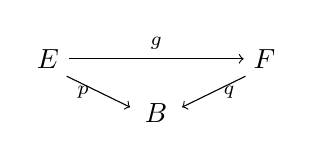
\begin{tikzpicture}[x=1.7em,y=1.4em]
  \node (E) at (0,1.4) {$E$};
  \node (F) at (4.6,1.4) {$F$};
  \node (B) at (2.3,0) {$B$};
  \draw[->] (E) -- node[above]{$\scriptstyle g$} (F);
  \draw[->] (0.4,0.95) -- node[left,pos=0.5]{$\scriptstyle p$} (1.75,0.15);
  \draw[->] (4.2,0.95) -- node[right,pos=0.5]{$\scriptstyle q$} (2.85,0.15);
\end{tikzpicture}
\end{center}
是一个\trFiberedEquivalence，当且仅当它是一个逐纤维等价，意即对每个\trElement{}
$b\colon 1\to B$，诱导的纤维间\trFunctor{} $g_{b}\colon E_{b}\to F_{b}$ 是一个%
\trEquivalence。
\end{proposition}

\begin{proof}
\trCocartesianFibration{}之间的一个\trEquivalence{}必然是逐纤维等价，故只需
证明其逆。由命题 10.2.2 与命题 10.2.1，若 $\mathcal{K}$ 是一个
$(\infty,1)$-\trCategory{}的\trInfinityCosmos{}而 $B$ 是 $\mathcal{K}$ 中的
一个∞-\trCategory，则底拟范畴\trFunctor{}诱导一个宇宙论\trBiequivalence{}
$(-)_{0}\colon\mathcal{K}_{/B}\Rightarrow\QCat_{/B_{0}}$。由推论 10.3.2，
这个宇宙论\trBiequivalence{}反射\trEquivalence；而由命题 10.1.4，
$(-)_{0}\colon\mathcal{K}\to\QCat$ 保持\trCocartesianFibration{}及其间的%
\trCartesianFunctor。于是，为证一个既是\trCartesianFunctor{}又是逐纤维等价的
$g\colon E\to F$ 是 $B$ 之上的一个\trEquivalence
$B_{0}$ 之上的一个\trEquivalence，为此我们验证：这个\trFunctor{}满足%
\cref{prop:fiberwise-equivalence-cartesian-functor}的前提。由%
\cref{obs:elements-of-underlying-qcat}，底拟范畴 $B_{0}$ 的诸\trElement{}与
∞-\trCategory{} $B$ 的诸\trElement{}双射地对应，而宇宙论\trFunctor{}
$(-)_{0}\colon\mathcal{K}\to\QCat$ 既保持诸纤维又保持诸\trEquivalence。如此
我们看到：$g_{0}\colon E_{0}\to F_{0}$ 对一切 $b\colon 1\to B_{0}$ 都是逐纤维
等价。由\cref{prop:fiberwise-equivalence-cartesian-functor}，这个\trFunctor{}%
定义一个\trFiberedEquivalence，从而 $g$ 亦然。
\end{proof}

\begin{corollary}\label{cor:discrete-cartesian-trivial-contractible}
在一个 $(\infty,1)$-\trCategory{}的\trInfinityCosmos{}中，一个离散%
\trCartesianFibration{}是一个\trTrivialFibration，当且仅当它的诸纤维是%
\trContractible。
\end{corollary}

\begin{proof}
若 $p\colon E\twoheadrightarrow B$ 是一个离散\trCartesianFibration，则 $p$
定义一个\trCartesianFunctor
\begin{center}
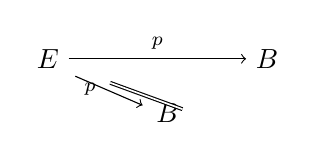
\begin{tikzpicture}[x=1.8em,y=1.4em]
  \node (E)  at (0,1.4) {$E$};
  \node (Bt) at (4.4,1.4) {$B$};
  \node (Bb) at (2.4,0) {$B$};
  \draw[->] (E) -- node[above]{$\scriptstyle p$} (Bt);
  \draw[->] (0.55,0.95) -- node[left,pos=0.45]{$\scriptstyle p$} (1.9,0.2);
  \draw[double] (1.25,0.78) -- (2.7,0.1);
\end{tikzpicture}
\end{center}
其余定义域是恒同的离散\trCartesianFibration。结论现在作为%
\cref{prop:fiberwise-equivalence-cosmos}之结果的一个特例而出现。
\end{proof}

\cref{prop:fiberwise-equivalence-cosmos}的结果可以延拓到诸\trModule{}：

\begin{corollary}[模的等价由逐纤维确定]\label{cor:module-equivalence-fiberwise}
在一个 $(\infty,1)$-\trCategory{}的\trInfinityCosmos{}中，从 $A$ 到 $B$ 的诸%
\trModule{} $E$ 与 $F$ 之间的一个映射
\begin{center}
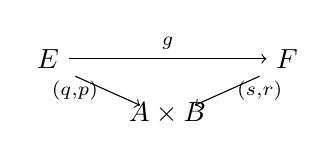
\begin{tikzpicture}[x=1.8em,y=1.4em]
  \node (E)  at (0,1.4) {$E$};
  \node (F)  at (4.8,1.4) {$F$};
  \node (AB) at (2.4,0) {$A\times B$};
  \draw[->] (E) -- node[above]{$\scriptstyle g$} (F);
  \draw[->] (0.55,0.95) -- node[left,pos=0.5]{$\scriptstyle(q,p)$} (1.85,0.2);
  \draw[->] (4.25,0.95) -- node[right,pos=0.5]{$\scriptstyle(s,r)$} (2.95,0.2);
\end{tikzpicture}
\end{center}
是一个\trEquivalence，当且仅当它是一个逐纤维等价，意即对每个\trElement{}
$a\colon 1\to A$ 与 $b\colon 1\to B$，诱导的纤维间\trFunctor{}
$g_{a,b}\colon E(b,a)\to F(b,a)$ 是一个\trEquivalence。
\end{corollary}

\begin{proof}
由引理 7.4.3 回忆起：左腿 $q\colon E\twoheadrightarrow A$ 与
$s\colon F\twoheadrightarrow A$ 是\trCocartesianFibration，而\trFunctor{} $g$
在它们之间定义一个\trCartesianFunctor。从而，由%
\cref{prop:fiberwise-equivalence-cosmos}，$g$ 是一个\trEquivalence，当且仅当对
每个\trElement{} $a\colon 1\to A$，拉回 $g_{a}\colon E(1,a)\to F(1,a)$ 是一个%
\trEquivalence。这些∞-\trCategory{}中的每一个都定义一个从 $1$ 到 $B$ 的%
\trModule，故再次由引理 7.4.3，拉回后的投影 $p\colon E(1,a)\twoheadrightarrow B$
与 $r\colon F(1,a)\twoheadrightarrow B$ 是\trCartesianFibration{}，而 $g_{a}$
在它们之间定义一个\trCartesianFunctor。由\cref{prop:fiberwise-equivalence-cosmos}
的对偶，这个\trFunctor{}是一个\trEquivalence，当且仅当对每个\trElement{}
$b\colon 1\to B$，纤维上的诱导作用
$g_{a,b}\colon E(b,a)\to F(b,a)$\footnote{原书此处印作
「$g_{a,b}\colon E(b,a)\to F(a,b)$」；按本条陈述（其纤维间\trFunctor{}作
$g_{a,b}\colon E(b,a)\to F(b,a)$）疑为 $F(b,a)$ 之误，此处径改。——译者注}
是一个\trEquivalence。这就证明了所述结果。
\end{proof}

这一结果的一个原型性特例，刻画了 $(\infty,1)$-\trCategory{}之间的诸%
\trAdjunction{}的单位或余单位：

\begin{corollary}\label{cor:counit-mapping-equivalences}
在一个 $(\infty,1)$-\trCategory{}的\trInfinityCosmos{}中，一支 2-\trCell{}
$\varepsilon\colon fu\Rightarrow\mathrm{id}_{A}$ 定义伴随 $f\dashv u$ 的余单位，
当且仅当诱导\trFunctor{}
$\qcor{\varepsilon\cdot f(-)}\colon\mathrm{Hom}_{B}(B,u)\to\mathrm{Hom}_{A}(f,A)$
——居于 $A\times B$ 之上——对每个\trElement{} $a\colon 1\to A$ 与
$b\colon 1\to B$ 都定义诸\trMappingSpace{}的等价
$\mathrm{Hom}_{B}(b,ua)\simeq\mathrm{Hom}_{A}(fb,a)$。
\end{corollary}

\cref{cor:module-equivalence-fiberwise}也可以应用于刻画诸 $(\infty,1)$-%
\trCategory{}之间的\trFullyFaithful{}\trFunctor{}与等价。

\begin{proposition}\label{prop:fully-faithful-pointwise}
在一个 $(\infty,1)$-\trCategory{}的\trInfinityCosmos{}中，一个\trFunctor{}
$f\colon A\to B$ 是\trFullyFaithful，当且仅当对一切\trElement{}
$a,a'\colon 1\to A$，其在诸\trMappingSpace{}上的作用
$f_{a,a'}\colon\mathrm{Hom}_{A}(a,a')\to\mathrm{Hom}_{B}(fa,fa')$ 定义诸%
\trDiscrete{}∞-\trCategory{}的一个等价。
\end{proposition}

\begin{proof}
第 3 章中的\cref{cor:fully-faithful}把一个\trFunctor{} $f\colon A\to B$ 定义为%
\trFullyFaithful，当且仅当诱导\trFunctor{}
$A^{2}\to\mathrm{Hom}_{B}(f,f)$——介于从 $A$ 到 $A$ 的诸\trModule{}之间——是
一个\trEquivalence。由\cref{cor:module-equivalence-fiberwise}，这成立当且仅当
这个映射定义一个逐纤维等价，而这恰好意味着：对一切\trElement{}
$a,a'\colon 1\to A$，其在诸\trMappingSpace{}上的作用
$f_{a,a'}\colon\mathrm{Hom}_{A}(a,a')\to\mathrm{Hom}_{B}(fa,fa')$ 定义诸%
\trDiscrete{}∞-\trCategory{}的一个等价。
\end{proof}

我们现在表明：$(\infty,1)$-\trCategory{}的等价恰好是那些在一个合适意义下逐点%
\trFullyFaithful{}且\trEssentiallySurjective\trFunctor。在文献 [102] 中，
Rezk 称这一结果为「拟范畴理论的基本定理」。我们的证明把综合技巧与解析技巧
混合起来：

\begin{theorem}[$(\infty,1)$-范畴理论的基本定理]\label{thm:fundamental-theorem}
在一个 $(\infty,1)$-\trCategory{}的\trInfinityCosmos{}中，一个\trFunctor{}
$f\colon A\to B$ 是一个\trEquivalence，当且仅当它
\begin{enumerate}[label=(\roman*)]
\item 是\textbf{\trFullyFaithful}：意即对一切\trElement{} $a,a'\colon 1\to A$，
  诱导映射
\[
\mathrm{Hom}_{A}(a,a')\longrightarrow\mathrm{Hom}_{B}(fa,fa')
\]
  是一个等价；并且
\item 是\textbf{\trEssentiallySurjective}：意即对一切 $b\colon 1\to B$，存在
  $a\colon 1\to A$ 与\trHomotopyCategory{} $\mathrm{h}B$ 中的一个%
\trIsomorphism{} $fa\cong b$。
\end{enumerate}
\end{theorem}

\begin{proof}
∞-\trCategory{}之间的一个等价 $f\colon A\Rightarrow B$ 诱导一个等价

同伦范畴的等价 $\mathrm{h}f\colon\mathrm{h}A\Rightarrow\mathrm{h}B$，以及介于从
$A$ 到 $A$ 的诸\trModule{}之间的一个等价
$A^{2}\simeq_{A\times A}\mathrm{Hom}_{B}(f,f)$——由第 3 章中的%
\cref{prop:pullback-equivalence}与\cref{prop:maps-between-commas}给出：
\begin{center}
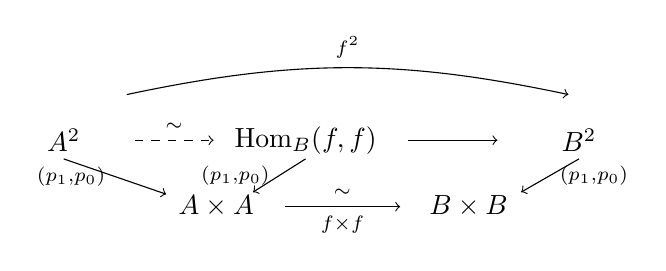
\begin{tikzpicture}[x=1.9em,y=1.5em]
  \node (a2)  at (0,1.6) {$A^{2}$};
  \node (hom) at (4.6,1.6) {$\mathrm{Hom}_{B}(f,f)$};
  \node (b2)  at (9.8,1.6) {$B^{2}$};
  \node (aa)  at (2.9,0) {$A\times A$};
  \node (bb)  at (7.7,0) {$B\times B$};
  \draw[->,dashed] (1.35,1.6) -- node[above]{$\scriptstyle\sim$} (2.85,1.6);
  \draw[->] (6.55,1.6) -- (8.25,1.6);
  \draw[->] (0,1.15) -- node[left]{$\scriptstyle(p_{1},p_{0})$} (1.95,0.3);
  \draw[->] (4.6,1.15) -- node[left]{$\scriptstyle(p_{1},p_{0})$} (3.6,0.35);
  \draw[->] (9.8,1.15) -- node[right]{$\scriptstyle(p_{1},p_{0})$} (8.7,0.35);
  \node at (5.65,0.8) {$\scriptstyle\lrcorner$};
  \draw[->] (4.2,0) -- node[above]{$\scriptstyle\sim$}
    node[below]{$\scriptstyle f\times f$} (6.4,0);
  \draw[->] (1.2,2.7) to[bend left=12] node[above]{$\scriptstyle f^{2}$} (9.6,2.7);
\end{tikzpicture}
\end{center}
本质满性是第一个等价的一个后果，而全忠实性则可沿 $A$ 的一对\trElement{}把第二
个等价拉回而得。

为证其逆，我们从把 $f$ 分解为一个\trEquivalence{}后接一个\trIsofibration{}开始。
两个因子都易于看出是逐点\trFullyFaithful{}且\trEssentiallySurjective，故
只需假设 $f\colon A\Rightarrow B$ 是一个\trIsofibration。我们现在的任务
是证明 $f$ 是一个\trTrivialFibration。在一个 $(\infty,1)$-\trCategory{}的%
\trInfinityCosmos{} $\mathcal{K}$ 中，命题 10.2.1 的宇宙论\trBiequivalence{}
$(-)_{0}\colon\mathcal{K}\Rightarrow\QCat$ 保持\trIsofibration{}并反射%
\trEquivalence。于是，为证一个\trIsofibration{} $f\colon A\Rightarrow B$
是一个\trTrivialFibration，只需证明底\trIsofibration{}
$f_{0}\colon A_{0}\Rightarrow B_{0}$ 是一个\trTrivialFibration——也就是
说，我们能够求解如下形式的\trLifting{}问题
\begin{rveq}\label{eq:trivial-fibration-lifting-fun}
\begin{tikzpicture}[x=1.9em,y=1.4em]
  \node (tl) at (0,1.4) {$\partial\Delta[n]$};
  \node (tr) at (5.6,1.4) {$\Fun(1,A)$};
  \node (bl) at (0,0) {$\Delta[n]$};
  \node (br) at (5.6,0) {$\Fun(1,B)$};
  \draw[->] (tl) -- (tr);
  \draw[right hook->] (0,0.95) -- (0,0.45);
  \draw[->,dashed] (1.0,0.25) -- (4.8,1.15);
  \draw[right hook-implies,double,double distance=0.6pt] (tr) -- node[right]{$\scriptstyle f_{0}$} (br);
  \draw[->] (bl) -- (br);
\end{tikzpicture}
\end{rveq}
对 $n\ge 0$。

在 $n=0$ 的情形，这条提升性质断言：当 $f_{0}\colon A_{0}\Rightarrow B_{0}$
是一个\trIsofibration{}时，「$f\colon A\Rightarrow B$ 是%
\trEssentiallySurjective」这一假设事实上蕴含
$f_{0}\colon A_{0}\Rightarrow B_{0}$ 在顶点上满射。由本质满性，对任何%
\trElement{} $b\colon 1\to B$，存在某个\trElement{} $a\colon 1\to A$ 使得
$fa\cong b$ 在 $\mathrm{h}B\coloneqq\mathrm{h}\Fun(1,B)\coloneqq\mathrm{h}(B_{0})$
中成立。现在，第 1 章中的\cref{cor:hc-isomorphism}蕴含：$B$ 的%
\trHomotopyCategory{}中的任何\trIsomorphism{}都可以由一个%
\trHomotopyCoherentIsomorphism{} $\qcInt\to\Fun(1,B)$ 来表示。选取一个%
\trElement{} $a\colon 1\to A$ 连同表示 $fa\cong b$ 的一个%
\trHomotopyCoherentIsomorphism{} $\beta\colon\qcInt\to\Fun(1,B)$，便定义出
如下\trLifting{}问题
\begin{center}
\begin{tikzpicture}[x=1.9em,y=1.4em]
  \node (tl) at (0,1.4) {$\varnothing$};
  \node (tm) at (3.0,1.4) {$1$};
  \node (tr) at (8.6,1.4) {$\Fun(1,A)$};
  \node (bl) at (0,0) {$1$};
  \node (bm) at (3.0,0) {$\qcInt$};
  \node (br) at (8.6,0) {$\Fun(1,B)$};
  \draw[->] (tl) -- (tm);
  \draw[->] (tm) -- node[above]{$\scriptstyle a$} (tr);
  \draw[right hook->] (0,0.95) -- (0,0.45);
  \node at (0.62,1.12) {$\scriptstyle\lrcorner$};
  \draw[right hook->] (3.0,0.95) -- (3.0,0.45);
  \draw[right hook-implies,double,double distance=0.6pt] (tr) -- node[right]{$\scriptstyle f_{0}$} (br);
  \draw[right hook->] (0.7,0) -- (2.45,0);
  \draw[->] (3.7,0) -- node[below]{$\scriptstyle\beta$} (6.4,0);
  \draw[->,dashed] (3.8,0.25) -- (7.9,1.15);
  \draw[->] (0.7,-0.8) to[bend right=15] node[below]{$\scriptstyle b$} (7.9,-0.8);
\end{tikzpicture}
\end{center}

它可以求解——沿\trIsofibration{}提升该\trIsomorphism{}即可。这就求解了
$n=0$ 情形的\trLifting{}问题 \eqref{eq:trivial-fibration-lifting-fun}。

把第 3 章中的\cref{prop:maps-between-commas}应用于左下方的交换图表，我们看到：诸\trModule{}之间的诱导映射是
一个\trIsofibration。
\begin{center}
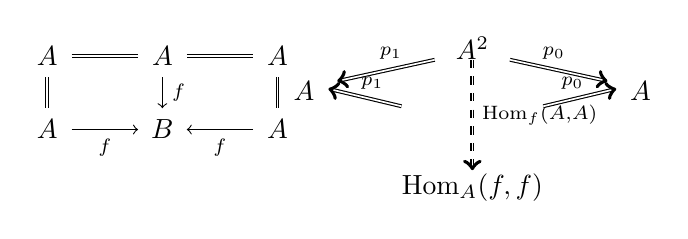
\begin{tikzpicture}[x=1.6em,y=1.4em]
  \node (a1) at (0,2.9) {$A$};
  \node (a2) at (2.6,2.9) {$A$};
  \node (a3) at (5.2,2.9) {$A$};
  \draw[double] (0.55,2.9) -- (2.05,2.9);
  \draw[double] (3.15,2.9) -- (4.65,2.9);
  \node (b1) at (0,1.0) {$A$};
  \node (b2) at (2.6,1.0) {$B$};
  \node (b3) at (5.2,1.0) {$A$};
  \draw[double] (0,2.35) -- (0,1.55);
  \draw[->] (2.6,2.35) -- node[right]{$\scriptstyle f$} (2.6,1.55);
  \draw[double] (5.2,2.35) -- (5.2,1.55);
  \draw[->] (0.55,1.0) -- node[below]{$\scriptstyle f$} (2.05,1.0);
  \draw[->] (4.65,1.0) -- node[below]{$\scriptstyle f$} (3.15,1.0);
  \node at (7.6,1.9) {$\rightsquigarrow$};
  \begin{scope}[shift={(9.6,0)}]
    \node (A2)  at (0,3.1) {$A^{2}$};
    \node (Al)  at (-3.8,2.0) {$A$};
    \node (Ar)  at (3.8,2.0) {$A$};
    \node (hb)  at (0,-0.5) {$\mathrm{Hom}_{A}(f,f)$};
    \draw[->,double,double distance=0.6pt] (-0.85,2.8) -- node[above,pos=0.45]{$\scriptstyle p_{1}$} (-3.05,2.25);
    \draw[->,double,double distance=0.6pt] (0.85,2.8) -- node[above,pos=0.45]{$\scriptstyle p_{0}$} (3.05,2.25);
    \draw[->,dashed,double,double distance=0.6pt] (0,2.8) -- node[right]{$\scriptstyle\mathrm{Hom}_{f}(A,A)$} (0,-0.05);
    \draw[->,double,double distance=0.6pt] (-1.6,1.6) -- node[above,pos=0.4]{$\scriptstyle p_{1}$} (-3.25,2.05);
    \draw[->,double,double distance=0.6pt] (1.6,1.6) -- node[above,pos=0.4]{$\scriptstyle p_{0}$} (3.25,2.05);
  \end{scope}
\end{tikzpicture}
\end{center}

由\cref{prop:fully-faithful-pointwise}，「$f$ 是逐点\trFullyFaithful」这一
假设——在诸纤维之间诱导等价
$f_{a,a'}\colon\mathrm{Hom}_{A}(a,a')\Rightarrow\mathrm{Hom}_{B}(fa,fa')$——蕴含：诱导
映射 $\mathrm{Hom}_{A}(f,f)\colon A^{2}\Rightarrow\mathrm{Hom}_{B}(f,f)$ 是一个%
\trEquivalence，从而在当前假设下是一个\trTrivialFibration。宇宙论\trFunctor{}
$(-)_{0}\colon\mathcal{K}\Rightarrow\QCat$ 把这个映射带为诸\trQuasiCategory{}%
之间的一个\trTrivialFibration，后者随之对 $n\ge 0$ 享有左下方所示的%
\trLifting{}性质：
\begin{center}
\begin{tikzpicture}[x=1.48em,y=1.7em]
  \node (tl) at (0,1.5) {$\partial\Delta[n]$};
  \node (tr) at (4.0,1.5) {$(A_{0})^{2}$};
  \node (bl) at (0,0) {$\Delta[n]$};
  \node (br) at (4.0,0) {$\mathrm{Hom}_{B_{0}}(f_{0},f_{0})$};
  \draw[->] (tl) -- (tr);
  \draw[right hook->] (0,1.05) -- (0,0.45);
  \draw[->,dashed] (0.9,0.25) -- (3.3,1.25);
  \draw[->] (tr) -- node[right,pos=0.35]{$\scriptstyle\mathrm{Hom}_{f_{0}}(A_{0},A_{0})$} (br);
  \draw[->] (bl) -- (br);
  \node at (8.0,0.75) {$\leftrightsquigarrow$};
  \begin{scope}[shift={(9.8,0)}]
    \node (tl2) at (3.6,1.8) [align=center]
      {$\partial\Delta[n]\times\Delta[1]$\\[-0.5ex]
       $\cup_{\partial\Delta[n]\times\partial\Delta[1]}$\\[-0.5ex]
       $\Delta[n]\times\partial\Delta[1]$};
    \node (tr2) at (12.4,1.8) {$A_{0}$};
    \node (bl2) at (3.6,0) {$\Delta[n]\times\Delta[1]$};
    \node (br2) at (12.4,0) {$B_{0}$};
    \draw[->] (tl2) -- (tr2);
    \draw[right hook->] (3.6,0.85) -- (3.6,0.4);
    \draw[->,dashed] (5.0,0.3) -- (11.6,1.45);
    \draw[->] (tr2) -- node[right]{$\scriptstyle f_{0}$} (br2);
    \draw[->] (bl2) -- (br2);
  \end{scope}
\end{tikzpicture}
\end{center}
经由例 A.6.14 中所给出的「逗号构造作为\trWeightedLimit{}」的描述，左上方的提升
性质穿过定义 A.6.5 的加权极限双变量伴随之 Leibniz 版本而转置，成为右上方所示的
提升性质，同样对 $n\ge 0$。

我们已经证明：$f_{0}\colon A_{0}\twoheadrightarrow B_{0}$ 也对包含
$\varnothing\hookrightarrow\Delta[0]$ 享有右提升性质。由于这个映射与 Leibniz
积包含 $(\partial\Delta[n]\hookrightarrow\Delta[n])\,\hat{\times}\,(\partial\Delta[1]\hookrightarrow\Delta[1])$
在超限复合、推出与收缩之下生成\trSimplicialSet{}的\trMonomorphism{}类，故由
「映射 $\mathrm{Hom}_{f_{0}}(A_{0},A_{0})$ 是一个\trTrivialFibration」这一事实
即知：$f_{0}\colon A_{0}\Rightarrow B_{0}$ 是一个\trTrivialFibration。
从而 $f\colon A\Rightarrow B$ 是一个\trTrivialFibration，此即所欲证。
\end{proof}

\subsection*{练习}

\begin{exercise}\label{ex:cartesian-lari-initial-elements}
用\cref{lem:opposite-qcat-biequivalence}证明\cref{prop:cocartesian-rari-terminal-elements}
与\cref{prop:fiberwise-equivalence-cartesian-functor}的对偶。
\end{exercise}

\begin{exercise}\label{ex:duals-other-results}
利用\cref{ex:cartesian-lari-initial-elements}中建立的对偶，陈述并证明本节其他
结果的对偶。
\end{exercise}

\begin{exercise}\label{ex:second-proof-absolute-right-lifting}
用\cref{cor:module-equivalence-fiberwise}给出%
\cref{prop:absolute-right-lifting-pointwise}(ii) 的第二个证明。
\end{exercise}


